% -*- mode: LaTeX; coding: utf-8; -*-

\chapter{Tiedon keruu ja esikäsittely}

Luvussa \ref{sec:lahtokohta} kuvailtiin tutkittavien lokitiedostojen
alkuperää ja tiedostomuotoa. Tässä luvussa tutustutaan
seikkaperäisemmin siihen, miten Ixonokselta saamamme palvelinloki on
järjestetty tiedostoihin ja millä tavoin tietoa on esikäsitelty
analyysiä silmällä pitäen. Käytetyt menetelmät soveltuvat pienin
muutoksin myös muiden Web-hotellien palvelinlokien esikäsittelyyn,
mikäli arkistointikäytänteet eivät suuresti poikkea tässä esitellystä.

Esimerkeissä käytetyt palvelinten ja palveluiden nimet ovat
kuvitteellisia, mutta rakenne vastaa tutkittua ympäristöä.

 % - Mistä data on peräisin?
 %    - Palvelun rakenteen kuvaus
 % - Millaista data on?
 %   - HTTP
 %   - Apachen logit
 % - Miten data on kerätty? (ohjelmistot ja verkkotopologia)
 %   - Yleisellä tasolla
 % - Mitä työkaluja on käytetty (Haskell ja PhasefulSplitter)
 % - Miten dataa on käsiteltu ja suodatettu?

\section{Tiedon rakenne}

Ixonoksen Web-hotelli on toteutettu siten, että yksittäiset palvelut on
sijoitettu jokaiselle palvelimelle. Ratkaisun taustalla on
kuormituksen tasaaminen. Erillinen järjestelmä huolehtii siitä, että
Internetistä tulevat kyselyt ohjataan tasaisesti eri
palvelimille. 

Taulukossa \ref{nimet} on esimerkki palveluiden ja
palvelinten nimeämisestä.

% Ei kannata ottaa esimerkkiä tästä taulukosta, tämä on vähän mutkikas.
\begin{table}[h]
\centering
\begin{tabular}{lll}
Palvelin && Palvelu \\
\cline{1-1}\cline{3-3}
dapper && buzz \\
edgy && rex \\
feisty && potato \\
&& hamm \\
&& slink \\
\end{tabular}
\caption{Palvelinten ja palveluiden nimeäminen.}
\label{nimet}
\end{table}

Lokitiedostot on sijoitettu hakemistorakenteeseen, jossa juuressa ovat
palvelinten nimien mukaiset hakemistot, joiden sisällä sijaitsevat
lokitiedostot, jotka on nimetään yhdistämällä palvelun nimi
päivämääräleimaan. Tiedostonnimessä käytetty päivämäärän muoto
noudattaa ISO 8601 -standardia~\cite{iso8601}. Tiedostot on pakattu
\texttt{gzip}-pakkausohjelmalla. Taulukossa \ref{tiedostot}
havainnollistetaan tiedostonnimien muodostumista.

\begin{table}[h]
\centering
\begin{tabular}{llll}
Palvelin & Palvelu & Päivämäärä & Tiedostonnimi \\
\hline
edgy & buzz & 14.6.2009 & \texttt{edgy/buzz.http.2009-06-14.gz}\\ 
dapper & potato & 2.7.2009 & \texttt{dapper/potato.http.2009-07-02.gz}\\
feisty & rex & 30.7.2009 & \texttt{feisty/rex.http.2009-07-30.gz}\\
\end{tabular}
\caption{Tiedostojen nimeäminen.}
\label{tiedostot}
\end{table}

Tässä mainittujen palvelinten lisäksi käytössä on ulkoinen
välimuistipalvelu, jonka kautta välitetään harvoin muuttuvia
resursseja, kuten kuvia. Valtaosa dataliikenteestä
välitetään palvelun kautta. Välimuistipalvelu toimii siten, että
mikäli pyydettyä resurssia ei löydy sen omasta muistista, se pyytää
sitä yhdeltä Web-hotellin palvelimista ja välittää vastauksen edelleen
asiakkaalle. Välimuistipalvelun käyttö ei kuitenkaan muilta osin
vaikuta palvelun rakenteeseen. Rakenne käy ilmi kuvasta
\ref{palvelinrakenne}.

\begin{figure}[htp]
\centering
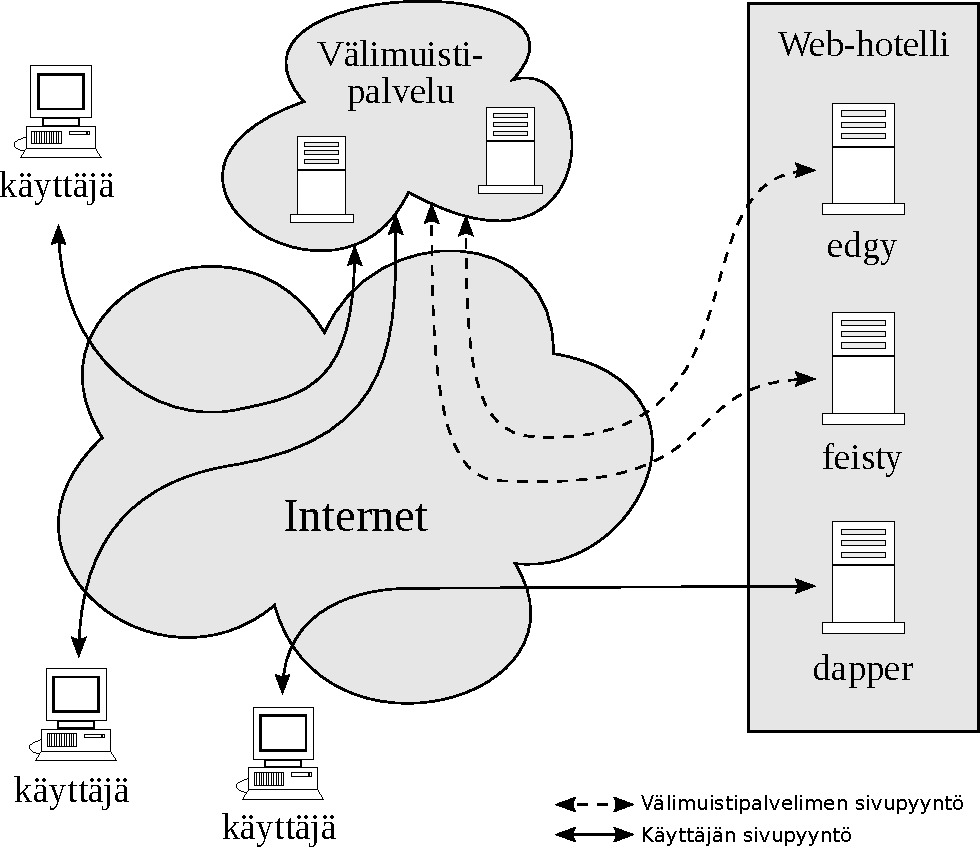
\includegraphics[width=12cm]{pics/palvelinrakenne.pdf}
\caption{Web-palvelun rakenne.}
\label{palvelinrakenne}
\end{figure}

\section{Tavoite}



\section{Esikäsittely}

\todo{Tästä luvusta puuttuu vielä tekstiä!}

Luvussa \ref{sec:lahtokohta} esiteltiin lokitiedostoissa käytetty
\textit{Combined Log Format} -muoto. Tiedosto on tekstimuotoinen,
joten se ei sellaisenaan sovellu analyysivaiheeseen, jossa käsitellään
klustereita. Osa palvelinlokin sisällöstä on myös analyysin kannalta
tarpeetonta ja nämä osat tulee suodattaa pois. Lisäksi yhteen
Web-palveluun liittyvät kyselyt ovat lisäksi jakautuneet useaan eri
tiedostoon eri palvelinten ja vuorokausien mukaisesti.

Esikäsittelijä on toteutettu osana tätä tutkimusta. Esikäsittelijä on
nimeltään \textit{PhasefulSplitter} ja se on toteutettu
Haskell-ohjelmointikielellä~\cite{haskell98}. Haskell tarjoaa
tehokkaat työkalut ohjelmakoodin rinnakkaistamiseen ja datan
sarjallistamiseen. \textit{PhasefulSplitter} on vapaa ohjelma ja sitä saa
levittää edelleen ja muuttaa Free Software Foundationin julkaiseman
GNU General Public Licensen (GPL-lisenssi) version 3~\cite{gplv3} tai (valinnan
mukaan) myöhemmän version ehtojen mukaisesti. Esikäsittelijä on
ladattavissa Internetistä osoitteesta \\
\url{http://iki.fi/zouppen/repo/phasefulsplitter.git}.

Sopivaa yksivaiheista parseria käyttämällä olisi mahdollista käsitellä
lähtödata suoraan analyysissä käytettävään muotoon. Käytännössä
kuitenkin datan esikäsittely kannattaa hoitaa useammassa vaiheessa,
jotta datassa olevat puuttuvat tai poikkeavat arvot voidaan huomioida
ja esikäsittelijää voidaan korjata suorittamatta koko ajoa uudelleen
alusta lähtien. Monivaiheinen esikäsittely helpottaa myös datan
käsittelyä jälkikäteen erilaisin menetelmin. Lisäksi sarjallistetut
tietorakenteet voidaan tarvittaessa anonymisoida, jolloin dataa
voidaan luovuttaa myös ulkopuoliseen käyttöön.

Tiedon käsittelyn helpottamiseksi tässä työssä käytetään esikäsittelyn
välivaiheet ja lopputulokset tallennetaan väliaikaistiedostoihin.
Relaatiotietokantaa ei käytetä, koska tietokantakyselyiden
rinnakkaistaminen osoittautui hyvin vaikeaksi verrattuna suoraan
tiedostoja käsittelevään toteutukseen.

Esikäsittely jakaantuu seuraavaat kolmeen vaiheeseen:

\begin{enumerate}
\item Tiedostolistan muodostaminen ja tiedostojen ryhmittely palveluittain.
\item Tiedostojen sisällön lukeminen ja muuntaminen tietorakenteeksi.
\item Tietorakenteiden jatkokäsittely.
\end{enumerate}

\subsection{Tiedostolistan muodostaminen}

Tekstipohjainen tiedostolista luetaan
\textit{PhasefulSplitter}-ohjelman ymmärtämään muotoon, jolloin
tiedostonnimet ryhmitellään palveluiden nimien perusteella. 

Luokittelun yhteydessä palvelinten nimet korvataan numeerisilla
viitteillä. Tätä varten asetetaan tiedestoon \texttt{server.map}
palvelinten nimet ja niitä vastaavat numeeriset viitteet. Viitteitä
voidaan hyödyntää myöhemmin, jos halutaan muuntaa analyysivaiheessa
kiinnostava havainto takaisin Apache-lokin riviksi. Tässä luvun
esimerkissä käytettävän tiedoston sisältö on esitelty listauksessa
\ref{servermap}

\begin{lstlisting}[language=MyHaskell,float=h,caption=Tiedoston server.map sisältö.,label=servermap,aboveskip=1cm]
[
      ("dapper",1)
    , ("edgy",2)
    , ("feisty",3)
]
\end{lstlisting}

Tiedostolista voidaan muodostaa
Linux-järjestelmässä seuraavalla tavalla:

\begin{lstlisting}[language=bashshell]
mkdir lists
find [[polku]] -iname '*.gz' | classifier lists/
\end{lstlisting} 

Ajon yhteydessä muodostuu hakemiston \texttt{lists} alle palveluiden
mukaan nimetyt tiedostot, joiden sisällä on palveluun kuuluvat
tiedostonnimet. Tiedostot ovat tekstimuotoon sarjallistettuja.

\subsection{Muuntaminen tietorakenteeksi}

Toisessa vaiheessa tekstimuotoiset lokitiedostot luetaan ja
käsitellään koneellisesti helpommin analysoitavaan muotoon. Tätä työtä
varten kehitetyssä tiedonkäsittelijässä lokitiedoston rivin eri kentät
palastellaan ja kyselyt sarjallistetaan tiedostoihin. Tietorakenne on
esitelty listauksessa \ref{entry}.

\lstset{language=MyHaskell}

\begin{lstlisting}[float=h,caption=Yhden lokirivin säilövä tietorakenne.,label=entry,aboveskip=1cm]
data Entry = Entry {
      info      :: LineInfo
    , ip        :: ByteString
    , date      :: UTCTime
    , method    :: ByteString
    , url       :: URL
    , protocol  :: ByteString
    , response  :: Integer
    , bytes     :: Integer
    , referer   :: ByteString
    , browser   :: ByteString
} deriving (Show,Eq)
\end{lstlisting}

Koska jatkokäsittely voidaan hoitaa säikeistettynä useammalle
prosessorille tai ytimelle, tässä vaiheessa sovellukselle tulee
ilmoittaa säikeiden määrä. Tiedon perusteella sovellus jakaa yhteen
palveluun liittyvän datan haluttuun määrään erillisiä tiedostoja. Jako
mahdollistaa tehokkaan jälkikäsittelyn, koska tiedostojen sisältöä on
mahdollista käsitellä myöhemmin samanaikaisesti.

Linuxin \texttt{xargs}-komennolla voidaan myös tämän vaihe suorittaa
rinnakkaistettuna, jolloin eri palveluihin kuuluva data voidaan
muuntaa samanaikaisesti. Mikäli eri palveluihin kuuluvien lokien datamäärä
vaihtelee, ei rinnakkaistamisesta kuitenkaan saavuteta täyttä hyötyä.

Alla olevassa esimerkissä esikäsitellään \texttt{lists}-hakemistosta
löytyvät tiedostolistat ja kirjoitetaan ne hakemiston \texttt{data}
alle. Korvaa listauksessa esiintyvä N tietokoneen prosessorien tai
ytimien määrällä. 

\begin{lstlisting}[language=bashshell]
ls lists/*| xargs -n 1 -I{} -P [[N]] apache2data [[N]] {} data/
\end{lstlisting}

Suoritusaika riippuu luonnollisesti koneen suorituskyvystä ja
lokitiedostojen määrästä. Tämän tutkimuksen yhteydessä suoritetussa 24
gigatavun ajossa 2,5 gigahertsin Intel Xeon -prosessorilla varustetussa
tietokoneessa tämän vaiheen suoritus kesti useita
prosessorivuorokausia.

\subsection{Parametrien N-grammianalyysi}

Palvelinlokissa olevista kyselyistä muodostetaan tietorakenne, jossa
yksi osa on kyselyn URL. Tässä vaiheessa tutkitaan URL-osoitetta
tarkemmin. Mikäli URL:n osana on parametreja, muodostetaan jokaisesta
parametrin arvosta 2-grammilistaus. Näin saadut 2-grammikartat
muodostetaan ja lopuksi ne tallennetaan matriisina tekstimuotoon
jatkokäsittelyä varten. Tiedostossa \texttt{ParameterAnalyzer.hs} on
määritelty vakiona, että lasketaan nimenomaisesti 2-grammit. Tätä
vakiota voi kuitenkin tarvittaessa muuttaa.

Ensimmäisessä ajossa selvitetään, mitkä mahdollisista 2-grammeista
ylipäätään esiintyvät aineistossa. Mahdollisia N-grammeja on yhteensä
$2^{8n}$ kappaletta, koska käsiteltävät merkkijonot koostuvat
Word8-tyypeistä (8-bittinen tavu). Säästääkseme muistia
analyysivaiheessa, selvitetään aluksi, millaisia 2-grammeja
aineistossa esiintyy ja jätetään taulukoimatta sellaiset 2-grammit,
jotka eivät esiinny lainkaan.

Jokaiselle resurssille muodostuu oma N-grammilistansa. Datan määrä
luonnollisesti riippuu käytettävästä aineistosta. Käyttämällämme
datalla taulukon kooksi muodostuu muutamia megatavuja (FIXME täsmällisesti).
Lopputulos on kuitenkin vain murto-osa alkuperäisen datamassan
suuruudesta.

N-grammianalyysin ensimmäinen vaihe suoritetaan menemällä halutun
palvelun mukaiseen hakemistoon ja suorittamalla seuraavan komennon:

\begin{lstlisting}[language=bashshell]
parameter_analyzer *.pf.gz +RTS -N
\end{lstlisting} 

Hakemistoon muodostuu ajon seurauksena tiedostot \texttt{ngrams.out}
ja \texttt{grams\_raw.txt}. Näistä ensimmäinen on binaarimuodossa ja
sisältää toisessa vaiheessa tarvittavan datan
binaarimuodossa. Toisessa tiedostossa on tekstimuodossa (Haskellin
show-muodossa) eri resurssien ja 2-grammien
esiintymistiheydet. Tekstimuotoista tiedostoa voidaan käyttää apuna
arvioitaessa, mihin resursseihin ja parametreihin kannattaa kiinnittää
jatkossa huomiota.

Tämän jälkeen voidaan suorittaa n-grammianalyysin toinen vaihe koko
palvelun sisältämälle datalle. Suoritetaan seuraava komento samassa
hakemistossa, missä ensimmäinen vaihekin suoritettiin:

\begin{lstlisting}[language=bashshell]
TODO
\end{lstlisting} 

Käyttämässämme datassa olevat kyselyiden parametrit sisältävät hyvin
samantyyppisiä arvoja, joten niistä muodostuu kohtuullisen
pieniulotteisia 2-grammitaulukoita. TODO kuinka pieniä? Tämän vuoksi
matriiseihin ei sovelleta satunnaisprojektiota.

TODO.

\section{Jatkokäsittely}

Lopuksi eri kenttien numeeriset ja
luokka-asteikolliset arvot klusteroidaan.

TODO
